\chapter{Análisis del ecosistema CVN y propuesta de solución}
\label{cap:ecosistema_cvn}

El Capítulo~\ref{cap:estado_arte} concluyó que una representación curricular
abierta debe combinar una separación clara entre modelo conceptual,
serialización y validación con una trazabilidad explícita hacia las fuentes
normativas del dominio. El presente capítulo aplica esa conclusión al caso
concreto de este Trabajo Fin de Grado. En primer lugar, se examina en detalle el
contenido real del paquete oficial de CVN empleado como fuente del proyecto. A
continuación, se identifican las limitaciones técnicas que dicho paquete
introduce cuando se pretende utilizarlo directamente como modelo interno de una
aplicación. Finalmente, a partir de ese análisis, se presenta la arquitectura
Open CVN que se desarrolla con más detalle en los capítulos siguientes.

\section{El paquete oficial CVN como fuente del proyecto}
\label{sec:ecosistema_paquete_oficial}

El Capítulo~\ref{cap:introduccion} ya situó a CVN como la norma española de
referencia para la presentación de información curricular de investigadores,
mantenida por FECYT~\cite{cvn_web}. Ese capítulo, sin embargo, se limitó a
introducir CVN como motivación del proyecto, sin describir el contenido técnico
del paquete que FECYT distribuye para su implementación. Esa descripción es el
punto de partida de este apartado.

El paquete oficial empleado como fuente de este trabajo no es un único fichero,
sino un conjunto heterogéneo de artefactos que puede organizarse en cuatro
capas complementarias. La primera capa es un manual de especificaciones técnicas
en formato PDF, orientado a lectura humana, que define el significado funcional
de cada campo curricular, su tipo de dato, su obligatoriedad y la tabla de
referencia asociada cuando corresponde. La segunda capa traduce ese mismo manual
a un fichero XML estructurado, pensado para su explotación automática en lugar
de su lectura directa. La tercera capa es un modelo en árbol que enlaza cada
código funcional del manual con las propiedades e indicadores concretos que
aparecen en un documento CVN real serializado en XML. La cuarta capa está
formada por los esquemas XSD que definen la forma legal de ese XML, incluyendo
un vocabulario extenso de tablas auxiliares codificadas como enumeraciones.

Junto a estas cuatro capas, el paquete incluye tres familias auxiliares que no
forman parte del núcleo mínimo de codificación, pero que resultan necesarias
para interpretar correctamente numerosas referencias del manual: un catálogo
normalizado de entidades e instituciones, una materialización en XML de buena
parte de las tablas del anexo de valores controlados junto con la codificación
de subtipos, y un tesauro jerárquico multilingüe de materias y palabras clave.
Sin estas familias auxiliares, una parte relevante de los campos del manual
quedaría referida a catálogos externos sin forma de resolverse dentro del propio
paquete.

La Tabla~\ref{tab:ecosistema_fuentes} resume, para cada una de estas fuentes, la
información principal que aporta y el uso concreto que recibe dentro del
proyecto.

\begin{table}[htbp]
  \centering
  \small
  \renewcommand{\arraystretch}{1.2}
  \begin{tabular}{p{0.24\textwidth} p{0.34\textwidth} p{0.30\textwidth}}
    \hline
    \textbf{Fuente} & \textbf{Información que aporta} & \textbf{Uso dentro del proyecto} \\
    \hline
    Manual de especificaciones técnicas (PDF) & Semántica funcional de cada campo curricular, tipo de dato y obligatoriedad & Referencia normativa para interpretar el significado de los códigos CVN \\
    Manual estructurado en XML & Catálogo del manual en forma parseable: código, nombre, tipo, obligatoriedad y tabla de referencia & Fuente principal para la extracción automática de metadatos funcionales \\
    Modelo en árbol XML & Enlace entre cada código funcional y las propiedades e indicadores del XML CVN real & Trazabilidad estructural entre el dominio funcional y la serialización XML \\
    Esquemas XSD del núcleo (documento, tipos comunes y tablas auxiliares) & Forma legal del XML final y vocabulario de tablas codificadas como enumeraciones & Generación reproducible de bindings estructurales y validación de forma \\
    Tablas de referencia y subtipos & Materialización en XML de gran parte del anexo de valores controlados y de la codificación de subtipos & Resolución de referencias auxiliares y evaluación de enumeraciones cerradas \\
    Catálogo de entidades & Registro normalizado de instituciones y entidades & Resolución de referencias de tipo registro \\
    Tesauro multilingüe & Vocabulario jerárquico de materias y palabras clave & Resolución de referencias de tipo tesauro \\
    \hline
  \end{tabular}
  \caption{Fuentes del paquete oficial CVN analizadas y su uso en el proyecto.}
  \label{tab:ecosistema_fuentes}
\end{table}

Estas fuentes no son intercambiables entre sí. El manual en PDF y su versión
estructurada en XML son la mejor base para entender \emph{qué significa} cada
campo, mientras que el modelo en árbol y los esquemas XSD explican \emph{cómo se
serializa} ese mismo campo dentro de un documento XML concreto. Esta distinción,
introducida aquí de forma descriptiva, es la que justifica más adelante por qué
la propuesta Open CVN separa explícitamente el análisis semántico del dominio de
su representación técnica en XML.

\section{El XML embebido en los documentos CVN}
\label{sec:ecosistema_pdf_embebido}

Además del paquete de especificación descrito en el apartado anterior, la
herramienta oficial de FECYT genera, para cada currículo, un documento en
formato PDF pensado principalmente para su presentación y lectura humana. Una
parte relevante de estos documentos conserva, embebido dentro del propio
fichero PDF, el XML CVN que dio lugar a su generación. Cuando ese XML embebido
existe y resulta accesible, constituye una fuente adicional de información
curricular ya estructurada, en lugar de un simple documento visual del que haya
que extraer texto de forma no estructurada.

Esta circunstancia tiene una implicación práctica directa para el procesamiento
automático de currículos ya existentes: un sistema que pretenda incorporar
currículos previamente generados por la herramienta oficial puede intentar, en
primer lugar, recuperar y validar ese XML embebido, y solo recurrir a mecanismos
menos deterministas cuando dicha extracción no sea posible. Este trabajo adopta
precisamente ese criterio de prioridad, cuyo desarrollo funcional completo se
presenta en el Capítulo~\ref{cap:formato_herramienta}.

\section{Limitaciones y dificultades técnicas detectadas}
\label{sec:ecosistema_limitaciones}

El análisis detallado del paquete oficial revela un conjunto de limitaciones
técnicas que, sin restar validez a la norma CVN, condicionan de forma directa
cualquier intento de utilizar sus artefactos como modelo interno de una
aplicación. Estas limitaciones se agrupan en cuatro tipos.

En primer lugar, existen discrepancias puntuales entre el XML canónico del
modelo en árbol y el esquema XSD que se supone que lo valida. El caso más
representativo aparece en dos indicadores concretos del modelo en árbol, que
incluyen un elemento hijo no declarado por dicho esquema. De los cientos de
indicadores del mismo tipo presentes en el documento, únicamente dos contienen
ese elemento adicional, y ambos hacen referencia al mismo valor de una tabla
auxiliar de tipos de calidad. Esta discrepancia impide que unas estructuras
generadas directamente desde el esquema puedan analizar por completo el XML
canónico, y obliga a tratar dicho XML como evidencia de origen que debe
registrarse explícitamente en lugar de forzarse a encajar en la forma legal
definida por el esquema.

En segundo lugar, ciertas construcciones del propio lenguaje de esquemas no se
trasladan de forma perfecta a estructuras de datos ejecutables. El mecanismo de
composición \textit{choice}, que en XSD permite declarar alternativas entre
varios elementos posibles, no siempre puede imponerse como una restricción de
exclusión mutua real sobre las estructuras generadas automáticamente a partir
del esquema. De forma similar, algunas cardinalidades mínimas declaradas en el
esquema no quedan garantizadas por dichas estructuras, y varios atributos se
generan con un tipo demasiado genérico, sin estructura interna definida. Estas
limitaciones son consistentes con una idea ya avanzada en el Capítulo
anterior: un esquema de validación describe la forma legal de un documento,
pero no captura por completo las reglas semánticas del dominio que representa.

En tercer lugar, no todas las tablas auxiliares del paquete se comportan como
enumeraciones cerradas. Algunas incluyen valores de tipo \emph{delegado} o
comportamiento abierto que impide tratarlas como un catálogo fijo sin perder
información, mientras que otras sí son suficientemente estables y compactas
para ese tratamiento. Determinar esta distinción exige examinar la evidencia
concreta de cada tabla en lugar de asumir un criterio uniforme para todas ellas.

En cuarto lugar, algunas referencias mencionadas en el manual funcional no
tienen una tabla equivalente clara dentro del resto del paquete, y las tres
familias auxiliares descritas en el apartado anterior presentan una deriva
histórica de empaquetado, con nombres de fichero que no siempre coinciden entre
la documentación de orientación y los artefactos realmente distribuidos. Esta
circunstancia obliga a resolver dichas familias mediante un mapeo consciente
del paquete, en lugar de asumir convenios de nombre fijos.

En conjunto, estas cuatro limitaciones evidencian un mismo problema de fondo:
la estructura XML del paquete oficial y el significado curricular que dicha
estructura pretende representar no están completamente alineados entre sí. La
Tabla~\ref{tab:ecosistema_limitaciones} resume estas limitaciones junto con la
respuesta de diseño que se adopta para cada una de ellas dentro de la
arquitectura Open CVN.

\begin{table}[htbp]
  \centering
  \small
  \renewcommand{\arraystretch}{1.2}
  \begin{tabular}{p{0.44\textwidth} p{0.44\textwidth}}
    \hline
    \textbf{Limitación detectada} & \textbf{Respuesta de diseño} \\
    \hline
    Discrepancias puntuales entre el XML canónico y su esquema de validación & Tratar el XML como evidencia de origen y registrar la discrepancia de forma explícita, sin forzar un análisis silencioso ni descartar el documento \\
    Construcciones XSD que no se trasladan de forma perfecta a estructuras ejecutables (\textit{choice} sin exclusión mutua, cardinalidades mínimas no garantizadas, atributos demasiado genéricos) & Confinar estas limitaciones a la capa estructural de bindings y no exponerlas como el contrato público de Open CVN \\
    Tablas auxiliares que no siempre son enumeraciones cerradas & Evaluar la elegibilidad de enumeración cerrada a partir de evidencia concreta de cada tabla, en lugar de un criterio uniforme asumido de antemano \\
    Referencias del manual sin tabla equivalente clara, y deriva de empaquetado entre familias auxiliares & Conservar estas referencias como no resueltas o parcialmente trazables en lugar de forzar una conversión con pérdida de información \\
    Separación insuficiente entre estructura XML y significado curricular & Introducir capas intermedias explícitas de normalización, política semántica y modelo conceptual antes de definir el formato final \\
    \hline
  \end{tabular}
  \caption{Limitaciones detectadas en el paquete oficial CVN y respuesta de diseño de Open CVN.}
  \label{tab:ecosistema_limitaciones}
\end{table}

Ninguna de estas limitaciones invalida la norma CVN ni el paquete distribuido
por FECYT, que cumplen adecuadamente su función original de interoperabilidad
documental. Lo que estas limitaciones muestran es que dicho paquete no puede
tomarse, sin mediación adicional, como el modelo interno definitivo de una
herramienta de gestión curricular. Esa mediación adicional es precisamente el
objeto de la propuesta de solución que se presenta a continuación.

\section{Propuesta de solución: la arquitectura Open CVN}
\label{sec:ecosistema_propuesta}

Copiar directamente la estructura del XML oficial como modelo interno de una
aplicación resolvería la interoperabilidad con CVN, pero trasladaría a dicha
aplicación todas las limitaciones descritas en el apartado anterior, y
mezclaría dos preocupaciones de naturaleza distinta: la interoperabilidad con
un formato de intercambio externo y el modelado semántico del dominio
curricular. Por este motivo, Open CVN no adopta el XML oficial como modelo
final, sino que lo trata como una fuente formal de la que se parte mediante un
proceso reproducible y explícitamente trazable.

Esta decisión no implica renunciar a la relación con CVN. Al contrario: la
propuesta exige conservar, para cada elemento del modelo final, evidencia
verificable de la fuente CVN de la que procede, de modo que la transformación
hacia un formato propio no suponga una pérdida de significado curricular. Esta
exigencia de trazabilidad se traduce en una arquitectura organizada por capas,
en la que cada capa añade una interpretación adicional sobre la capa anterior
sin descartar la relación con el paquete oficial. La Figura~\ref{fig:ecosistema_separacion}
representa esta idea de forma esquemática.

\begin{figure}[htbp]
  \centering
  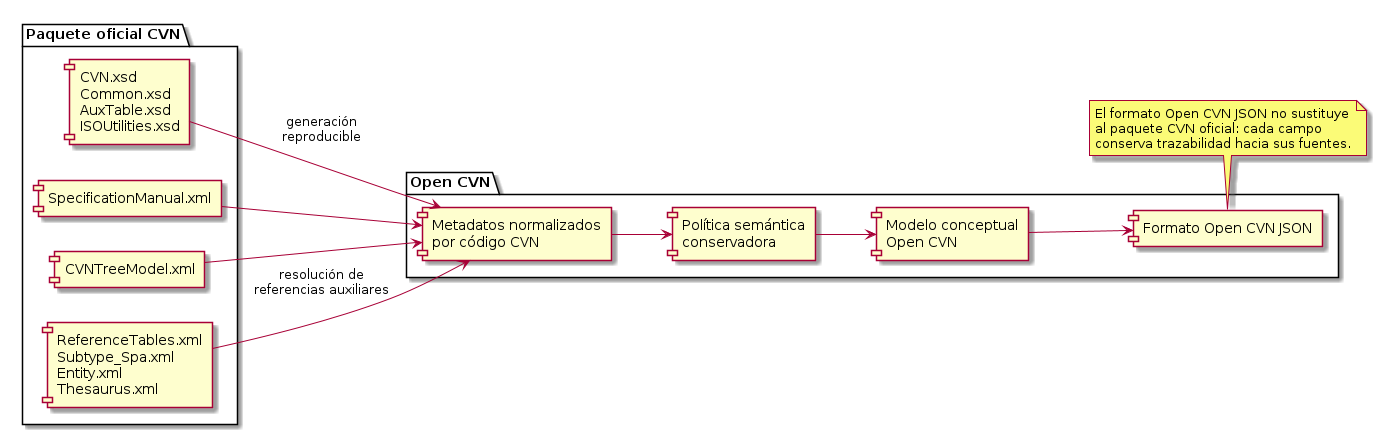
\includegraphics[width=0.95\textwidth]{figs/open_cvn_source_separation.png}
  \caption{Separación entre el paquete oficial CVN y la arquitectura Open CVN.}
  \label{fig:ecosistema_separacion}
\end{figure}

Como muestra la Figura~\ref{fig:ecosistema_separacion}, el paquete oficial
completo, incluidas sus familias auxiliares, se convierte en primer lugar en
metadatos normalizados por código CVN, un paso que unifica en una única
estructura la información dispersa entre el manual, el modelo en árbol y las
fuentes auxiliares. Sobre esos metadatos normalizados actúa una política
semántica conservadora, que decide de forma explícita y trazable cómo debe
interpretarse cada campo: como texto, fecha, número, enumeración cerrada,
catálogo abierto, referencia a una entidad, término de tesauro o referencia no
resuelta, entre otros casos. El resultado de esta política alimenta un modelo
conceptual de dominio que ya no depende de la estructura concreta del XML
CVN, y que constituye la base a partir de la cual se deriva finalmente el
formato Open CVN JSON descrito en el Capítulo~\ref{cap:formato_herramienta}.

Este modelo conceptual se representa mediante diagramas de clases UML, tal y
como se anticipó en el Capítulo~\ref{cap:estado_arte}. La
Figura~\ref{fig:ecosistema_uml_overview} muestra una vista compacta de dicho
modelo, en la que un documento Open CVN se organiza en metadatos, un bloque de
currículo y un espacio de extensión, y en la que ese bloque de currículo se
subdivide en áreas conceptuales del dominio académico e investigador. Los
nombres de clase de esta vista coinciden deliberadamente con las claves
técnicas del formato Open CVN JSON, de modo que la figura sirva también como
puente directo hacia la estructura raíz que se detalla en el
Capítulo~\ref{cap:formato_herramienta}.

\begin{figure}[htbp]
  \centering
  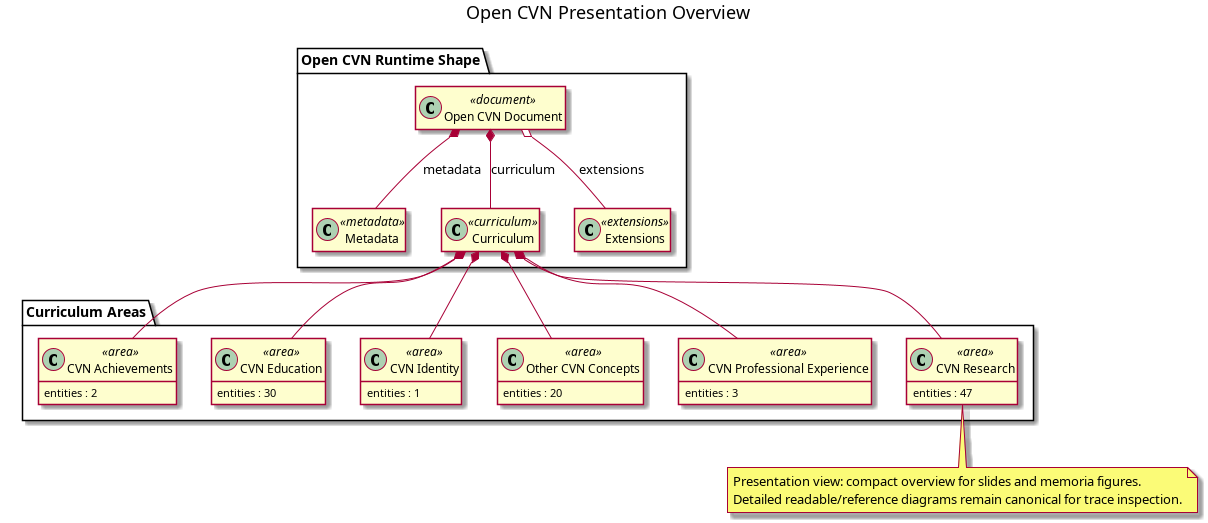
\includegraphics[width=0.95\textwidth]{figs/open_cvn_presentation_overview.png}
  \caption{Vista UML compacta del esquema conceptual de Open CVN, con el número de conceptos identificados por área curricular.}
  \label{fig:ecosistema_uml_overview}
\end{figure}

Sobre esta base conceptual y de trazabilidad se construyen finalmente los
mecanismos que hacen operativa la propuesta: un formato Open CVN JSON validable
y extensible, y un conjunto de utilidades de análisis, validación e importación
que, junto con una herramienta local de gestión, demuestran que la
representación definida puede emplearse en flujos reales de trabajo curricular.
Esta herramienta local cumple una función demostrativa del enfoque, mientras
que la aportación principal de la propuesta reside en la arquitectura de
representación, normalización y trazabilidad descrita en este apartado.

\section{Alcance y exclusiones}
\label{sec:ecosistema_alcance_exclusiones}

El análisis anterior permite delimitar con precisión qué garantías ofrece
realmente la arquitectura Open CVN frente al ecosistema CVN del que parte.

Se automatizan con garantías reproducibles los siguientes elementos:

\begin{itemize}
  \item La generación de la capa estructural desde los esquemas oficiales.

  \item La normalización de metadatos por código CVN a partir del manual y
  del modelo en árbol.

  \item La resolución de referencias auxiliares cuando existe evidencia
  suficiente en el paquete.

  \item La aplicación de la política semántica conservadora.

  \item La generación del modelo conceptual y del formato Open CVN JSON a
  partir de dicho modelo.
\end{itemize}

Se mantienen como mapeo parcial, y así deben entenderse, los siguientes
elementos:

\begin{itemize}
  \item La interpretación de tablas auxiliares sin evidencia suficiente para
  una enumeración cerrada, que permanecen documentadas como abiertas o
  pendientes de revisión.

  \item La incorporación de currículos CVN ya existentes en formato XML, que
  se resuelve mediante un mapeo semántico de los elementos reconocidos del
  documento en lugar de una conversión completa y garantizada de cualquier
  XML CVN posible.
\end{itemize}

Quedan documentadas explícitamente como limitaciones o trabajo futuro:

\begin{itemize}
  \item Las referencias del manual sin tabla equivalente clara en el resto
  del paquete.

  \item La deriva de empaquetado entre familias auxiliares.

  \item La ausencia de una garantía formal de que el modelo conceptual
  capture la totalidad de las reglas de negocio implícitas en el manual
  funcional.
\end{itemize}

Ninguna de estas exclusiones se oculta: todas ellas se retoman de forma
explícita en la discusión de garantías del
Capítulo~\ref{cap:evaluacion}.

En conjunto, el análisis realizado en este capítulo justifica por qué Open CVN
no se limita a reproducir la estructura XML de CVN, sino que introduce una
arquitectura propia, trazable y validable a partir de ella. El Capítulo
siguiente describe la metodología de trabajo seguida y detalla la arquitectura
general por capas que materializa esta propuesta.
